\documentclass[a4paper,10pt, twocolumn]{article}
\usepackage{amsmath}
\usepackage{graphicx}
\usepackage[font={small,it}]{caption}
\renewcommand*\sfdefault{phv}
\usepackage{listings}
\lstset{
    language=R,
    basicstyle=\ttfamily
}

\begin{document}

\title{Evolution of Cooperation}
\author{Alun Meredith}
\maketitle

\begin{abstract}
In this paper we test the reproducibility of Powers' work \cite{Paper} on individual selection for cooperative group formation. In which Powers et. al. build a model to show that selection can not only operate in favour of cooperative individuals but selection can act on the environmental conditions which enable evolution to show the conditions which favour cooperation are evolvable despite being initially selected against. 

We then expand on this model exploring a critique that the binary model may be the source of many of the features observed and hypothesising a coevolutionary algorithm style arms race in a more continuous system. However we observe consistent decrease in selfishness despite the environmental conditions selecting for it, supporting Powers' arguement that "any component of selection on structuremodifying traits that is due to social behaviour must be in the direction of increased cooperation" \cite{Thesis}. 
\end{abstract}
\section{Introduction}
Cooperation can be defined as individuals taking some behaviour which doesn't directly benefit themselves in order to benefit the group as a whole; often tied to the idea that cooperative individuals may look for long term rewards at the expense of short term rewards. 

It is possible to try and explain cooperation through other mechanisms such as product of communication for intelligent animals. Or when the organism lives long enough to see the yield of cooperation within the time-frame of reproductive cycles cooperation improves immediate fitness so can be considered an optimal action in the time scale evolution acts upon. However cooperative behaviour is observed through many different levels of biological complexity and lifespans such as bacteria moderating their consumption of a limited resource \cite{Bacteria1,Bacteria2,Bacteria3,Bacteria4}. Through examples like these it can be inferred cooperation may be an evolved trait. 

The idea that cooperation can emerge as an evolutionary trait is not a trivial one. One of the core features of evolution is that selection acts upon what is immediately beneficial regardless of the future so individuals with higher immediate benefit will be selected for. Therefore greedy individuals maximising immediate gains will be selected for. 

To produce an evolutionary model which allows for the emergence of cooperative behaviour the positive effect of cooperating must outweigh the selective pressure to be greedy. Consider two isolated populations of individuals with no method of variation, one of greedy individuals and one of cooperative ones. The cooperative population would consume a limited resource more efficiently than a group population of only greedy individuals and therefore have higher fitness than the greedy population. Therefore it can be said that spatial structures, like isolated groups can allow cooperative behaviour to thrive \cite{Bacteria1,Bacteria2,Bacteria3,SpatialStructure}. 

The example above only worked by denying variation, especially through mutation to occur. This is because the presence of a single greedy individual in the cooperative group would corrupt the entire group to be cooperative by yielding the rewards of the cooperative groups actions while not suffering the reduced growth rate of the cooperative individuals. It has been proposed that continuously breaking up the groups and reforming them can offset the emergence of greedy mutations by creating some groups with no greedy individuals \cite{GroupSelection1,GroupSelection2,GroupSelection3}. 

It can be considered that the balance of cooperative to greedy individuals therefore is based on the between individual selection to produce greedy individuals and the between group selection to produce cooperative groups. 


The paper tries to produce conditions allowing cooperation to be selected for despite being initially selected against. In addition it allows the conditions which allow for cooperation themselves to be selected for by having an allele governing the size of the group each individual is placed in. With larger groups having less sampling error and therefore lower chance to have none/few greedy individuals. 

\subsection{Model}

The model takes the above concepts having populations of individuals form isolated groups and then grow based on their consumption of a limited resource shared to each group before dispersing and reforming the group every $(t)$ generations. 

The individuals in the model do not mutate and asexually reproduce, creating copies of themselves. Additionally the fitness of the individual is dictated by their ability consume a limited resource which is shared with individuals in the group.

There are genotypes of two binary loci. The first gene codes if the individual is greedy or cooperative, with greedy individuals requiring a larger amount of the resource to reproduce $(C)$, but also taking a larger proportion of the resource. The second loci dictates the size of the group the individual will be placed in when group formation occurs.  

The four genotypes are initially distributed evenly before being randomly sampled without replacement into groups of their preferred size any remaining individuals are discarded, which should have negligible effect for large population size. This produces groups with variance in their ratio of greedy and cooperative individuals due to sampling error. The groups are left to grow for $t$ generations before the population is normalised back to $N$ individuals and re-sampled into new groups. This cycle is repeated until $T$ generations have transpired.  

During each generation the genotypes grow in number and a fraction of them die ($K$). Each group is given a total amount of resource $(R)$ based on the size of the group. Large groups are given slightly more resource per individual than small groups to ensure large groups are initially selected for. 

The share of the groups resource each individual gets is based on the product of their growth rate and consumption rate relative to the other individuals in the group such that (\ref{eq:individualResource}) shows the amount of resource each individual will receive: 

\begin{align}
	r_i = \frac{G_iC_i}{\sum_j(G_jC_j)}R
	\label{eq:individualResource}
\end{align}

The consumption rate $C$ represents the amount of resource required to reproduce whereas the growth rate $G$ represents a weight for the amount of resource that phenotype takes in combination with consumption rate. So the number of times an individual reproduces is $\frac{r}{C}$. We can aggregate these changes to show the change in number of individuals belonging to a genotype $n_i$ in one generation, defined in (\ref{eq:genotypePopChange}). 

\begin{align}
	n_i(t+1) = n_i(t) + \frac{r_i}{C_i}- Kn_i
	\label{eq:genotypePopChange}
\end{align}

\begin{table}
\begin{tabular}{|l l |l|}
\hline
\textbf{Parameter} & & \textbf{Value} \\
\hline 
Growth rate (cooperative) & $G_c$ & 0.018 \\ \hline
Growth rate (selfish) & $G_s$ & 0.02 \\ \hline
Consumption rate (cooperative) & $C_c$ & 0.1 \\ \hline
Consumption rate (selfish) & $C_s$ & 0.2 \\ \hline
Population size & $N$ & 4000 \\ \hline
Number of generations & $T$ & 120 \\ \hline
Generations between groups & $t$ & 4 \\ \hline
Death rate & $K$ & 0.1 \\ \hline
Resource per group (large) & $R_l$ & 50 \\ \hline
Resource per group (small) & $R_s$ & 4 \\ \hline
\end{tabular}
\caption{Parameters used to reproduce Powers' findings \cite{Paper}}
\label{table:parametersReproduction}
\end{table}

\subsection{Reproduction}
The reproducibility of Powers' results have been tested \cite{Paper}, starting with the analysis of equilibrium states as a function of the parameters \textit{initial group size} and \textit{time spent in groups before mixing} ($t$).
 
\begin{figure}[ht]
	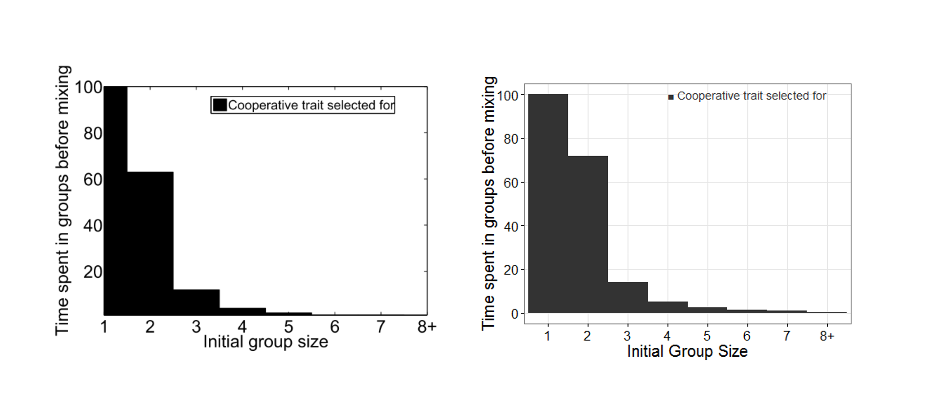
\includegraphics[width=\linewidth]{Figure1.png}
	\centering
	\caption{Equilibrium state of cooperative and greedy individuals as a function of initial group size and number of generations before mixing. Black regions show parameter combinations which select for cooperative trait; white areas for greedy trait. Left graph shows the original \cite{Paper} and right graph shows the reproduction.}
		\label{fig:Figure1}
\end{figure}

In figure \ref{fig:Figure1} we can see the same general shape in both Powers' and the reproduction graphs however there is some variance. The reproduction appears to systematically favour cooperative individuals slightly, most noticeably when the initial group size is two. Part of this could be explained by sampling error the reproduction only had 5 repetitions which could lead to some noticeable variance. However the difference in the two results appears systematic, one hypothesis for this is the way in which rounding is treated in both algorithms. The reproduction model aggregates decimals until after the groups are about to be reformed. By doing this artefacts caused by rounding thresholds in the small group size are far less likely. It is not known how Powers et. al. treats rounding in their model and was the biggest barrier to a perfect reproduction while building the model. 

The purpose of this figure is to find appropriate values for group size, ensuring the large group favours greedy individuals while the small group favours the cooperative individual. It is interesting that the small group was chosen to be size 4 with time between group mixing also 4 as this point is on or very close to an equilibrium point in Powers' reproduction. While it does favour cooperative individuals it would be safer to pick a value not on the equilibrium threshold.   

\begin{figure}[ht]
	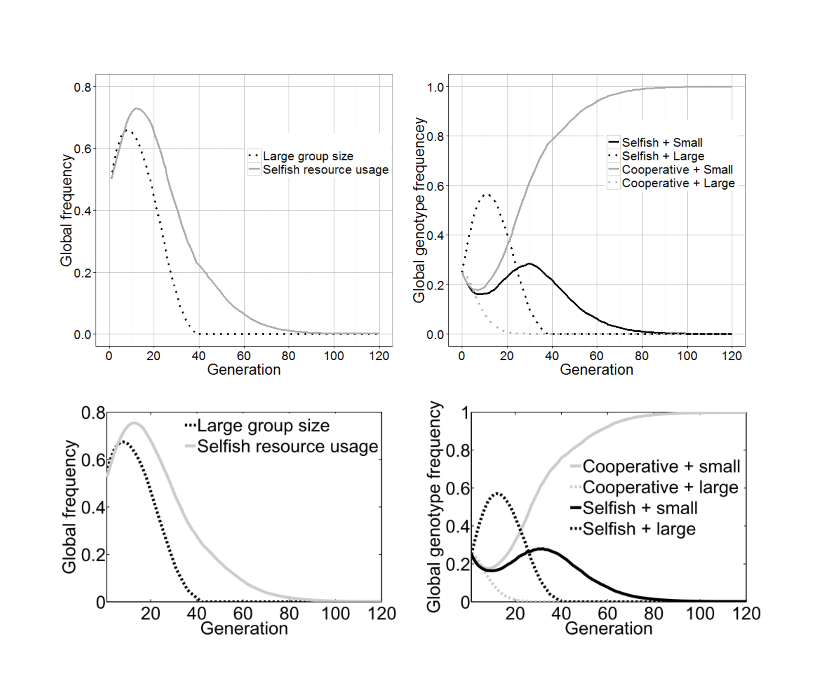
\includegraphics[width=0.9\linewidth]{Figure2.png}
	\centering
	\caption{Left hand plots shows the prevalence of each allele over time. Right hand plots shows the prevalence of each genotype over time. Top images show the original \cite{Paper}, bottom plots the reproduction.}
		\label{fig:Figure2}
\end{figure}

Figure \ref{fig:Figure2} from Powers' paper has also been reproduced. Here the differences between the reproduction and original are far more subtle and hard to identify. It appears as though the slight differences in construction which lead to figure \ref{fig:Figure1} being different have little impact on the overall dynamics of the system. 

Figure \ref{fig:Figure2} (right) shows how the different genotypes change frequency over time. As expected from fig:\ref{fig:Figure1} the selfish large genotype outcompetes the cooperative and large, while the cooperative and small outcompetes the selfish and small. In addition due to the extra resource given to the large group size the selfish large genotype grows much more rapidly at first until the population of cooperative and large individuals on which it was exploiting becomes extinct. At this point they too quickly become extinct leaving the cooperative and small genotype to flourish. The selfish and small genotype lasts much longer than the other dominated genotypes, because there is such a proportion of cooperative individuals each selfish individual has a larger advantage than in an even environment narrowing the gap between the two but ultimately still decreasing in population. 

In essence the above model is a competitive co-evolutionary model as the fitness of each individual is based only on their ability to compete with the other individuals in the population for a fixed resource, for example if a slightly more greedy phenotype was introduced under the same conditions you would expect the current selfish phenotype to be dominated by that individual as it is out-competed.

Powers' shows a model for which selection acts on the conditions which produce cooperative behaviour i.e. the favoured group size to produce cooperative behaviour despite being initially selected against. While it achieves this there is no inclusion of variation in the model, in particular no mutation which is surprising considering the purpose of using Wilson's trait group aggregation and dispersal method is to counter the effects of mutation in the population. Although similar models have been shown to work with mutation \cite{Thesis}

\section{Extension}

For the extension of this Paper we consider in more detail some of the limitations of Power's model. In Powers' thesis it is argued that "any component of selection on structuremodifying traits that is due to social behaviour must be in the direction of increased cooperation" \cite{Thesis}. We would like to test probe this hypothesis in more detail. Consider in figure \ref{fig:Figure2} the reason for the selfish and large phenotype to become extinct was that it no longer had less selfish individuals to exploit. We therefore hypothesise that the model will fail upon introducing a pseudo-continuous set of cooperative traits with mutation. Here there will be a non-binary distribution of cooperation in individuals so that in cases where selfishness is rewarded selfish individuals can continue to exploit the more cooperative individuals in their distribution. 

Making the analogy to a co-evolutionary model where it is expected the cooeprative trait will experience an arms race until it reaches the ceiling. It is this point we see in Powers' model similar to disengagement when there is no longer a more cooperative part of the population to exploit. During this arms race efficiency of consumption ($C$) would continue to deteriorate so we could expect a crash premature to reaching the ceiling. 

Consider an adaptation to Powers' model for figure \ref{fig:Figure2}. The individuals still have a loci with two traits for either large or small group size but 11 traits for cooperation. The values for consumption rate and growth rate scale linearly between the selfish and cooperative values in table \ref{table:parametersReproduction}. Before redistributing the population to groups allow random mutation of the cooperative loci up or down 1 step along the chain at a rate of $M = 0.1$.


\section{Results}
In this section we reproduce figures \ref{fig:Figure1} and \ref{fig:Figure2} for our new model. Exploring the conditions chosen in figure \ref{fig:Figure1} to find the areas of dominance of different levels of greed. The parameters for $C_i$ used is the sequence from $0.1 - 0.2$ by $0.01$ and for $G_i$ is the sequence from $0.018 - 0.02$ by $0.002$. Population size, $N$ has also been reduced to 1000 to improve computing performance. 

After redistributing the population to the 11 factors of greed figure \ref{fig:extensionFig2} showing the change in dominant genotype over time shows some notable similarities and differences to fig.\ref{fig:Figure1}. The general structure of the dark cooperative levels (Greed = 1 or 2) is very similar to the binary equilibrium states so it can be concluded that the conditions supporting highly cooperative action are consistent. 

The level of cooperation increases again after the initial group size of 5. This effect is very subtle, with only 5 repeat runs taken there could be significant sampling error here and would need exploring in more detail with a larger variety of parameters. However this does indicate an effect that ever increasing group sizes may not be uniforms detrimental to cooperativity supported by those parameters, especially when time between mixing kept low.

\begin{figure}[ht]
	\includegraphics[width=0.9\linewidth]{extensionEquilibriumPlot.png}
	\centering
	\caption{Equilibrium state of cooperative levels as a function of initial group size and number of generations before mixing. Black regions show parameter combinations which select for cooperative trait.}
		\label{fig:extensionFig2}
\end{figure}


\begin{figure}[ht]
	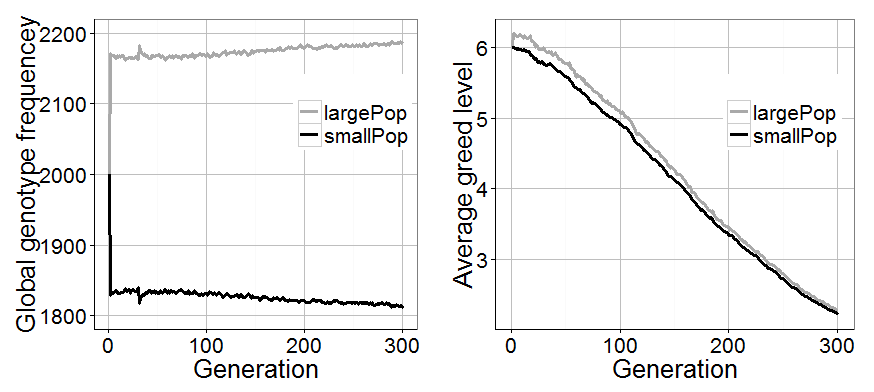
\includegraphics[width=0.9\linewidth]{extenstionFigure1.png}
	\centering
	\caption{Beep Boop}
		\label{fig:extensionFig1}
\end{figure}

The initial jump at the beginning in the first generation is likely an artefact of the code, having explored some potential causes the discarding of group sampling accounts for 0.5\% difference which cannot cause the discrepancy observed. The jump is formed in the initial growth stages and it is not clear if this in an artefact of the code or real because as a rule of thumb step functions don't exist in nature but a possible explanation is that the populations quickly adapt to the increased resource given to the large groups as the ratio between the group sizes at this point of 1.17:1 is close to the ratio between resource per individual of 1.2:1. 

In contrast to the binary model the genotype frequency for group size is roughly stable with no large changes. While the large population does increase slowly over time, it is possible that given enough generations a similar pattern to the binary model could be observed. 

Strikingly the average greed level from 1 (cooperative) to 11 (selfish) systematically decays over time for both large and small population. This effect is uniform for both the large population and small population despite the cooperative bias for small group size. 

It appears that the within group competition which benefits greedy individuals is being suppressed by the variety of different cooperation levels. An example of this is that in the 11 factor model, a single individual with the same level of greed as the binary model exploits the rest of the group to a lower level because the expected level of the group is approximately half way between the cooperative and selfish levels of the binary model.  

\begin{figure}[ht]
	\includegraphics[width=0.9\linewidth]{figure5.png}
	\centering
	\caption{Showing the different genotype frequencies of each genotype in the large group size over time}
		\label{fig:figure5}
\end{figure}

Observing figures \ref{fig:figure5} we observe similar effects to the binary model where "greedy" individuals initially peak but then crash leaving the cooperative factors of 1,2 and 3 to ultimately dominate. The final distribution becomes quite ordered by the initial 20 generations appears chaotic. Very high greed levels such as 8 + have very small peaks presumably due to the low efficiency of those levels combined with the average selfishness of population never reaching high numbers. The individuals which take advantage of the current population trade off efficiency and resource share. It appears that level 5 has the best combination of these variables however as the average selfishness decreases it shifts this ideal level down lower. While the same factors in play in the binary model eventually allow the cooperative genotypes to do well. 
\section{Conclusion}


While we haven't explored the limits of different conditions or run the model simulation for long enough to provide certainty in our results. We have shown support for the hypothesis of cooperation from social niche construction in spite of conditions such as group size selecting against it. 

We hypothesised an arms race increasing greediness as the ideal level of greed is only slightly above the average of the population due to decreased efficiency so individuals would have to be slightly more and more greedy  but observed the opposite where the average greed of the population slowly deteriorates shifting the ideal level of greed to capitalise on this down. Reinforced by the maintained high population of level 2 selfishness in the population despite trends of increased cooperation over time. 

\newpage
\onecolumn
\begin{thebibliography}{9}

  \bibitem{Paper}
  Simon T. Powers, Alexandra S. Penn, Richard A. Watson,
  \emph{Individual Selection for Cooperative Group Formation},
  Proceedings of the 9th European Conference on Artificial Life,
  (2007),
  585-594.
  
  \bibitem{Bacteria1}
  Pfeiffer, T., Schuster, S., Bonhoeffer, S.,
  \emph{Cooperation and competition in the evolution of ATP-producing pathways},
  Science \textbf{292}(5516),
  (2001),
  504-507.

  \bibitem{Bacteria2}
  Pfeiffer, T., Bonhoeffer, S.,
  \emph{An evolutionary scenario for the transition to undiferentiated multicellularity},
  PNAS \textbf{100}(3),
  (2004),
  2751-2760.
  
  \bibitem{Bacteria3}
  Kreft, J.U., 
  \emph{Biofilms promote altruism.},
  Microbiology \textbf{150},
  (2004),
  2751-2760.
  
  \bibitem{Bacteria4}
  Kreft, J.U., Bonhoeffer, S.,
  \emph{The evolution of groups of cooperating bacteria and the growth rate versus yield trade-off},
  Microbiology \textbf{151},
  (2005),
  636-641,
  
  \bibitem{SpatialStructure}
  Nowak, M.A., May, R.M,
  \emph{The spatial dilemmas of evolution},
  International Journal of Bifurcation and Chaos \textbf{3}(1),
  (1993),
  35-78,

  \bibitem{GroupSelection1}
  Wilson, D.S,
  \emph{A theory of group selection},
  PNAS \textbf{72}(1),
  (1975),
  143-146,
  
  \bibitem{GroupSelection2}
  Wilson, D.S,
  \emph{The Natural Selection of Populations and Communities},
  Benjamin/Cummings,
  (1980),
  
  \bibitem{GroupSelection3}
  Wilson, D.S,
  \emph{The Evolution and Psychology of Unselfish Behaviour},
  Harvard University Press, Cambridge, MA \textbf{3}(1),
  (1998),
  35-78,    
 
  
  \bibitem{Thesis}
  Simon T. Powers,
  \emph{Social nice construction: evolutionary explanations for cooperative group formation},
  University of Southampton, School of Electronics and Computer Science,
  Doctral Thesis, 
  186pp,
  (2010),
  
\end{thebibliography}
\section{Appendix}
The following code is written in the R language. 
\subsection{Appendix 1. Header file for reproduction}
This header file contains he major algorithmic functions to reproduce Powers' model. 
\lstinputlisting{reproductionHeader.r}
\subsection{Appendix 2. Script for reproducing figure 1.}
This script reproduces figure 1 of Powers' paper. The code for the graph is also included. The script is adapted from the reproduction of figure 2 script (appendix 3.)
\lstinputlisting{reproductionScriptForEquilibriumState.r}
\subsection{Appendix 3. Script file for reproducing figure 2.}
This file runs the functions described in the header in order to produce figure 1 and figure 2 in Powers' paper. The code for plotting the graphs is also present. 
\lstinputlisting{reproductionScript.r}
\subsection{Appendix 4. Header file for extension}
This header file contains the major algorithmic functions for the extension. It inherits many of its features from Appendix 1, adapting the same core algorithm for variable cooperation levels. 
\lstinputlisting{extensionHeader.r}
\subsection{Appendix 5. Script for extension}
This script contains code to produce figures [COMPLETE THIS DESCRIPTION]
\lstinputlisting{extensionScript.r}
\subsection{Appendix 6. Script for extension including mutation}
\lstinputlisting{extensionScript2.r}
\subsection{Appendix 7. Script for plotting Figure 3}
\lstinputlisting{extensionPlot1.r}
\subsection{Appendix 8. Script for plotting Figure 4}
\lstinputlisting{extensionEquilibriumPlot.r}



\end{document}
